
%\cleardoublepage
\section{Simulation von Fußgängern mit Social Force}\label{sec:SocialForce}

Da das Fahrzeug auf Gehwegen bzw. in Fußgängerzonen zum Einsatz kommen soll, befasst
sich dieser Abschnitt mit der Simulation von Fußgängern, die sich entweder
alleine oder in Gruppen bewegen. Mithilfe des \emph{Social Force} Modells
\cite{helbig1995socialforce} können die Bewegungen
der einzelnen Fußgänger mit additiven Kräften in Form von 2D Vektoren beschrieben
werden. Das ursprüngliche Modell kann durch zusätzliche Kräfte zur Umsetzung
von Gruppendynamiken \cite{moussaid2010groupssf} und der Interaktion mit Fahrzeugen
\cite{machines11020268} erweitert werden.

\subsection{Grundlagen Social Force}
Im Social Force Modell bestimmen Anziehungs- und Abstoßungskräfte die Richtung,
in die die einzelnen Fußgänger laufen. Pro Fußgänger wird eine gewichtete Summe
aller auf ihn wirkenden Kräfte gebildet, um die angestrebte Laufrichtung zu bestimmen.
Anschließend werden die resultierenden Kräfte in träge Bewegungen umgesetzt, die
die Fußgänger auf ihre angestrebten Gehgeschwindigkeiten beschleunigen und anschließend
auch halten, bis schließlich am Ziel abgebremst wird.\\

Die \emph{Desired Force} ist eine anziehende Kraft, die durch den Vektor von der
Position des Fußgängers zum Ziel beschrieben wird und somit den Fußgänger geradlinig
in Richtung des Ziels bewegt. Zur Vermeidung von Kollisionen wird der Fußgänger
mittels \emph{Obstacle Force} von Hindernissen abgestoßen, was durch das virtuelle
Potentialfeld $F = - \frac{\partial}{\partial p} dist(o, p)^{-2}$ der reziprogen Distanz
zwischen dem Fußgänger $p$ und dem Hindernis $o$ modelliert wird, wie in Abbildung
\ref{img:ObstacleForce} zu sehen ist.
Des weiteren beschreibt die \emph{Social Force} sowohl die Neugier der Fußgänger,
sich von anderen Fußgängern angezogen zu fühlen, als auch eine gewisse Abstoßung
gegenüber Fremden zu empfinden, wenn diese zu nahe kommen.
Durch die Differenzen der Bewegungsvektoren und Positionen zweier Fußgänger bewegt
eine anziehende Kraft die Fußgänger aufeinander zu. Kollisionen werden durch eine
abstoßende, orthogonale Kraft vermieden, sobald sich die Fußgänger zu nahe kommen,
sodass sich die Fußgänger gegenseitig ausweichen.\\

\begin{figure}[h]
  \centering
  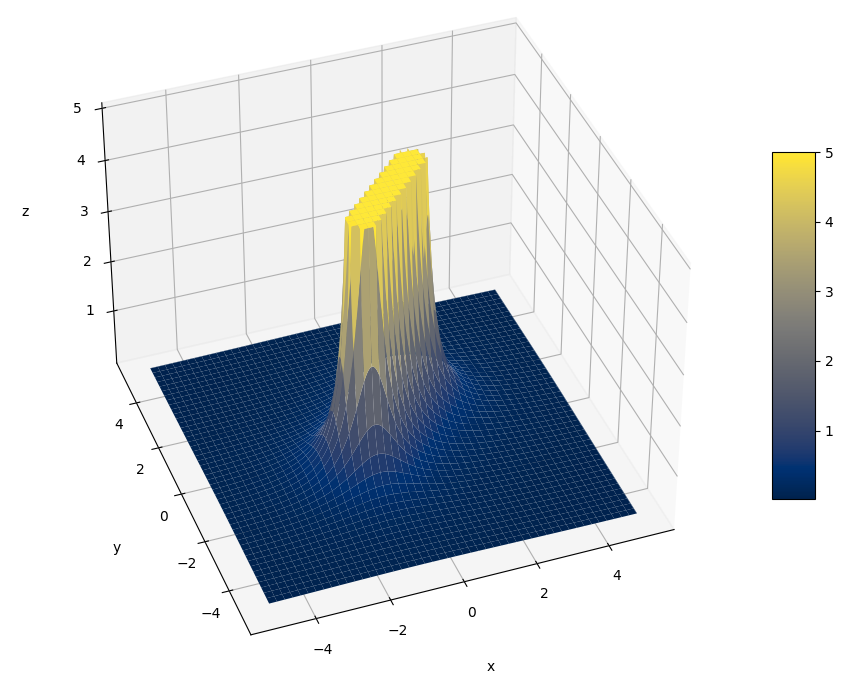
\includegraphics[width = 0.65\textwidth]{imgs/obstacle_repulsive_field}
  \caption{Potentialfeld der auf die Fußgänger wirkenden Abstoßungskraft von Hindernissen.
  Die x- und y-Achse entsprechen der modellierten 2D Ebene, die z-Achse repräsentiert
  die Stärke des Potentialfelds, das um das Hindernis wirkt. Bei der abstoßenden Kraft
  handelt es sich um die negative Magnitude bezüglich der Fußgängerposition.}
  \label{img:ObstacleForce}
\end{figure}

\subsection{Social Force mit Gruppen}
Bisher wurde nur die Modellierung einzelner Fußgänger betrachtet, die sich unabhängig
voneinander bewegen. Da aber ca. 70\% aller Fußgänger in Gruppen von ca. 2-4 Fußgängern
unterwegs sind \cite{moussaid2010groupssf}, wird das Social Force Modell
entsprechend um abstoßende und anziehende Kräfte erweitert, um Gruppendynamiken
zu beschreiben.\\

Anhand einiger Experimente wurde bei Gruppen häufig beobachtet, dass sich Gruppenmitglieder
in einer orthogonalen Linie zur Laufrichtung anordnen. Mittels orthogonaler Abstoßung
vom und gleichzeitiger Anziehung zum Gruppenzentrum, kann ein entsprechender Effekt
erzielt werden, was durch die \emph{Group Repulsive Force} und \emph{Group Cohesive Force}
umgesetzt wird.
Die \emph{Group Gaze Force} modelliert hingegen das Bedürfnis, sich während der Fortbewegung
als Gruppe mit Augenkontakt zu unterhalten. Äußere Gruppenmitglieder laufen daher
etwas vorne weg, was zur typischen V-Form führt, falls genügend Platz vorhanden ist.

\subsection{Simulation des Ausweichverhaltens bezüglich Fahrzeugen}
Nun sind die Fußgänger zwar in der Lage, untereinander und mit Hindernissen
zu interagieren, aber ignorieren bisher völlig das Fahrzeug. In der Realität würden
Fußgänger aber sehr wohl einem herannahenden Fahrzeug ausweichen, sofern sie dieses
rechtzeitig wahrnehmen können. Daher wird eine abstoßende Kraft zwischen Fahrzeug
und Fußgängern definiert, die das Fahrzeug als gewöhnliches Hindernis betrachtet,
dem die Fußgänger ausweichen müssen.\\

\begin{figure}[h]
  \centering
  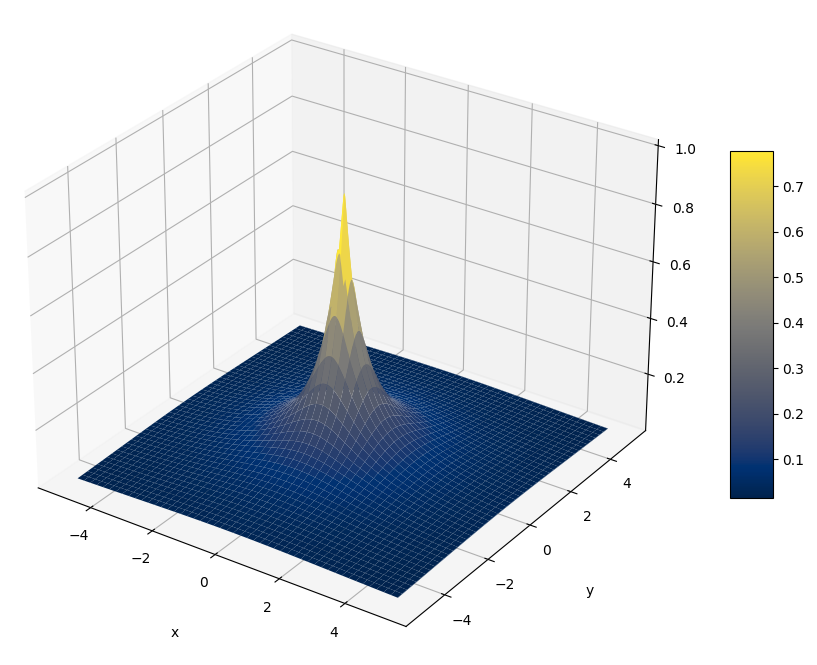
\includegraphics[width = 0.65\textwidth]{imgs/robot_repulsive_field}
  \caption{Potentialfeld der auf die Fußgänger wirkenden Abstoßungskraft von Fahrzeugen.
  Die x- und y-Achse entsprechen der modellierten 2D Ebene, die z-Achse repräsentiert
  die Stärke des Potentialfelds, das um die Position des Fahrzeug wirkt. Bei der
  abstoßenden Kraft handelt es sich um die negative Magnitude bezüglich der Fußgängerposition.}
  \label{img:PedRobotForce}
\end{figure}

Die \emph{Ped-Robot Force} wird ähnlich zur Abstoßung von Hindernissen als virtuelles
Potentialfeld umgesetzt, was durch die partielle Ableitung
$F = - \frac{\partial}{\partial p} dist(v, p)^{-2}$ der reziprogen Distanz zwischen
Fußgänger $p$ und Fahrzeug $v$ beschrieben wird, wie in Abbildung \ref{img:PedRobotForce}
dargestellt. Dies führt dazu, dass Fußgänger einem stehenden Fahrzeug auf einer
elliptischen Bahn ausweichen. Ein Beweis der Berechnungsformel liegt im Appendix bei.

\subsection{Mögliche Erweiterungen}
Für die Simulation zusätzlicher Verkehrsteilnehmer gibt es ebenfalls Modelle anhand
von Social Force. Dies ermöglicht beispielsweise die Steuerung von E-Scootern
\cite{liu2022scootersf} oder anderer Fahrzeuge \cite{huynh2014modelling} mittels
Social Force. Entsprechende Ansätze werden jedoch im Folgenden nicht weiter thematisiert,
da nur die Interaktion zwischen einem steuerbaren Fahrzeug und Fußgängern betrachtet werden soll.
Es wäre jedoch denkbar, per Social Force gesteuerte Fahrzeuge zu einem späteren Zeitpunkt
der Simulation hinzuzufügen, sofern die Modellierung derartiger Interaktionen mit der
autonomen Fahrsoftware sinnvoll erscheint.
